\chapter{Method}

\begin{comment}
Describe the pipeline used to generate NeRFs

- Capture (video, image, polycam, etc.)
- Process (COLMAP, or direct extraction from e.g. Polycam)
    - Configuration of COLMAP
- Train (Different models)
    - Configuration of model
- Render (Real-time rendering vs. slow rendering)
- Evaluate (PSNR, SSIM, LPIPS)
- Export

- Pipelines created
    - Pipeline to test 
\end{comment}

\section{Nerfstudio}
With the magnitude of different published methods regarding NeRF, some with corresponding source code and some not, it's not trivial to compare them on self-captured data. In the experiments, I have leveraged an open-source project named Nerfstudio. It is an API that streamlines the creation, training, and visualization of NeRFs. The components that make up NeRFs are modularized in a way that allows interpretable implementation of different NeRF methods. In addition, it ships with implemented versions of some of the most important published methods to date for real-world captures; NeRF, mip-NeRF, and instant-NGP.

\section{Nerfacto}
Nerfstudio also provides its own method dubbed "Nerfacto". The method isn't published work, but leverages techniques from several other published methods which have proved to work well for real data captures. The techniques used in Nerfacto result in a method that strikes a great balance between quality and speed. Most of the techniques highlighted by Nerfacto have already been discussed in \autoref{chap:relatedwork}, but I'll recap and elaborate on a few here.

\textbf{Camera pose refinement}, as described in \autoref{sec:camera-pose-refinement} is a technique proposed to reduce the impact of imperfect camera poses. It's a very effective measure to reduce cloudy artifacts and increase the sharpness and overall quality of the resulting 3D representation.

\textbf{Per image appearance conditioning}, as described in \autoref{sec:appearance-embeddings}, is a technique that allows the NeRF to process and represent 3D scenes with variable lighting, exposures, weather, and post-processing effects. In Nerfacto, the appearance embedding is a vector of size 32, which is concatenated with the viewing direction before it's passed through the MLP.

\textbf{Hash encodings} were proposed in \cite{muller_instant_2022}. This parametric encoding differs in how spatial data is represented. In the original NeRF paper, the location \textbf{x} is represented by a positional encoding. With the multiresolution hash encoding, the location \textbf{x} is represented in a hash table by a linear interpolation of its closest vertices at multiple resolutions. This parametric encoding has several advantages in terms of computational effectiveness, resulting in several magnitudes of increased training and inference speed. Although you impose a larger memory cost by allocating several hash tables, the number of required parameter-updates per backpropagation is severely reduced. In Nerfacto, 16 hash tables with $2^{19}$ rows, each storing a feature vector of size 2, are allocated. The subsequent MLP has a very low capacity, with only one hidden layer containing 64 neurons. An overview of the multiresolution hash encoding can be seen in \autoref{fig:instant-ngp-hash-encoding}.

%The only difference is essentially how spatial data is represented, i.e. parametric encoding. Instant-NGP encodes spatial data at multiple resolutions using hash tables, thereof the name multiresolution hash tables. During backpropagation, the MLP's weights and the feature vectors in the hash tables are both updated.
%In a fully connected MLP, every weight and bias must be updated on back-propagation. With parametric encodings, only a very small number of feature vectors must be updated. Also, by reducing the size of the MLP, such parametric models can be trained to convergence much faster without sacrificing approximation quality. You trade a larger memory footprint by allocating hash tables, but in return you have to update a far lower number of trainable parameters per back-propagation, leading to an increased training and inference speed.

\begin{figure}[h]
    \centering
    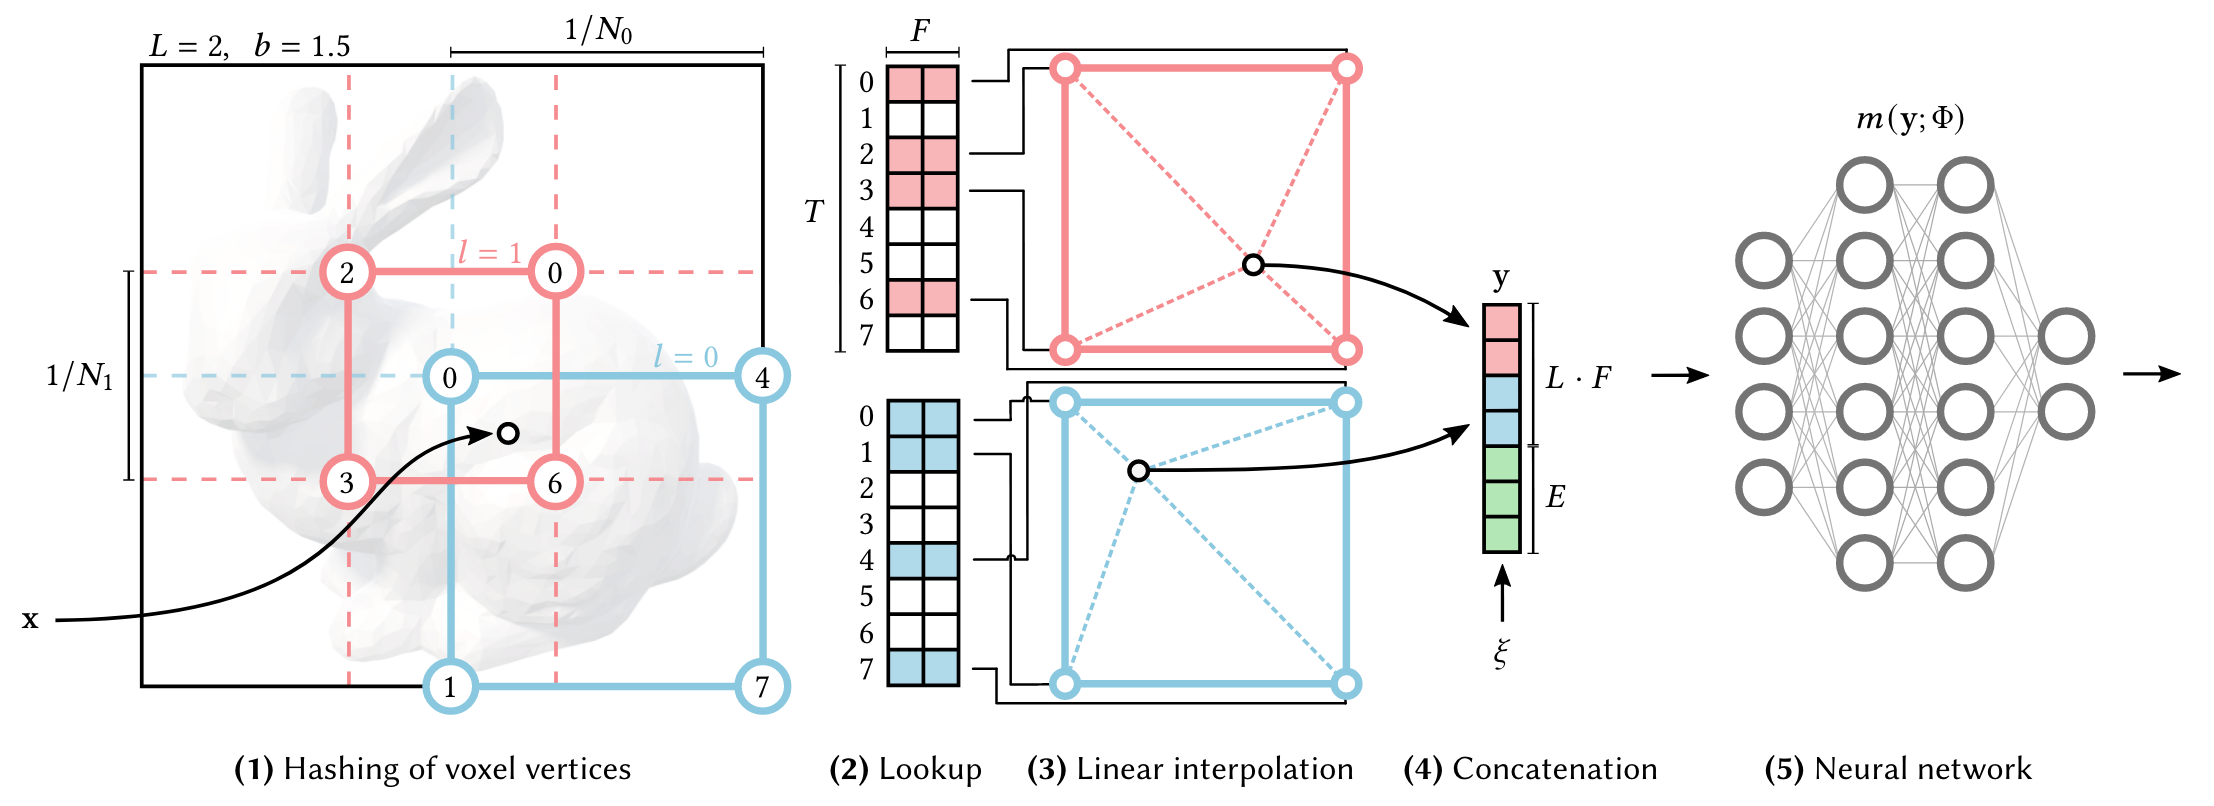
\includegraphics[width=1.0\textwidth]{figures/instant-ngp-hash-encoding.png}
    \caption{Illustration of the multiresolution hash encoding in 2D, Figure 3 \cite{muller_instant_2022}.}
    \label{fig:instant-ngp-hash-encoding}
\end{figure}

\textbf{Proposal sampling} is a sampling technique discussed in \autoref{sec:mipnerf360}. Nerfacto extends the proposal sampler used in mip-NeRF 360 by utilizing two density functions implemented as small fused-MLP with hash encodings \cite{muller_instant_2022}. This provides accurate and fast density estimations.

\textbf{Scene contraction}, as described in \autoref{sec:mipnerf360}, is a technique proposed in \cite{barronMipNeRF360Unbounded2022} to extend mip-NeRF to support unbounded scenes.

\section{Capture}
%- Video, image, polycam, etc. ✅
The different datasets have primarily been captured with an iPhone 13 Pro Max. The iPhone features three lenses that enable captures ranging from ultra-wide to telephoto. Using the ultra-wide option has proved helpful in the pipelines where COLMAP has to be leveraged as it captures more of the scene and more easily enables overlap between the frames. The resulting NeRF-renderings haven't seemed distorted. When capturing video or images for a NeRF it's important that the scene is well-lit, that you capture non-blurry images, and that there are no transient objects present.

Polycam is a "LiDAR \& 3D Scanner for iPhone \& Android". It has multiple settings for performing photogrammetry and LiDAR scans, but most importantly it enables export of images with corresponding camera poses. This is very useful as Nerfstudio has created an integration that reads the camera poses generated by Polycam and transforms it into Nerfstudio's data format. This enables skipping COLMAP entirely from the pipeline. Polycam doesn't support wide camera options, resulting in the need to manually record more of the scene.
%The quality of the camera poses are relatively good.

\section{Process}
%- COLMAP, or direct extraction from e.g. Polycam 
%- Configuration of COLMAP
The data processing step for constructing a NeRF are usually the same across different models. It's a step for creating the data set of images with corresponding camera poses and is comprised of creating a set of images from a video, scaling the images to a preferred size, and lastly utilizing an algorithm to extract the corresponding camera poses. All the experiments in this paper leverage Nerfstudio which has its own data processing pipeline API that includes support for video, images, and Polycam-data. For video input, FFMPEG\cite{tomar2006converting} is first used to grab image frames from the video at specified densities, by default ~300 frames. When a set of images is acquired, the images are scaled down in fractions of the original image size. The scaling of the images is done as it's been demonstrated that training on images larger than 1600px along the longest dimension has diminishing returns. COLMAP is then used for extracting the camera poses from the set of input images. The choice of matching algorithm, as discussed in \autoref{sec:sfm}, is primarily the only setting you have to tweak for COLMAP.

%COLMAP and FFMPEG \cite{tomar2006converting} are the main data processing tools. FFMPEG is used to grab image frames from the video at specified densities, by default ~300 frames. COLMAP is then used for extracting the camera poses from a set of input images. The choice of matching algorithm, as discussed in \autoref{sec:sfm}, is primarily the only setting you have to tweak for COLMAP.
%Most of the experiments use the default number of frames and the default COLMAP matching algorithm.

\section{Train}
%- Configuration of model
The training has been conducted with different models, varying amounts of data, and for different scenes. All the configurations have been adjusted with Nerfstudio's API.

\section{Render}
%- Real-time rendering vs. slow rendering
In order to render the scenes, a trained NeRF and a camera path is required. In Nerfstudio, a camera path can simply be created in their real-time rendered viewer. The camera path can later be exported and used across models trained on the same data to qualitatively compare them.


\section{Evaluate}
%Evaluation scripts


\section{Pipelines for testing}
%Discuss the different pipelines I've created to test different methods against each other.